\documentclass[10pt]{beamer}
\usepackage[english]{babel}
\usepackage[utf8]{inputenc}
\usepackage[T1]{fontenc}
\usepackage{helvet}


%-------------------------------------------------------
% INFORMATION IN THE TITLE PAGE
%-------------------------------------------------------

\newcommand{\cstitle}{\textbf{Bioinformatics against COVID-19}}
\subtitle[]{Bioinformatics Research Group}
\newcommand{\cscourseCode}{1005155}
\newcommand{\csauthor}{MSc. Vicente Machaca Arceda}
%\institute[UNSA]{Universidad Nacional de San Agustín de Arequipa}
\newcommand{\csemail}{vmachacaa@unsa.edu.pe}
\newcommand{\instituteabr}{UNSA}
\newcommand{\nameUp}{ICC Fase 1}
\date{\today}
\title[\cscourseCode]{\cstitle}
\author{\csauthor}
%%%%%%%%%%%%%%%%%

%-------------------------------------------------------
% CHOOSE THE THEME
%-------------------------------------------------------
\def\mycmd{0} % CS THEME
\def\mycmd{1} % MYTHEME
%-------------------------------------------------------

\if\mycmd1
	\usetheme[]{Feather}
	\newcommand{\chref}[2]{	\href{#1}{{\usebeamercolor[bg]{Feather}#2}} }
\else
	\usepackage{csformat}
\fi

\newcommand{\1}{
        	\setbeamertemplate{background}{
        		
\includegraphics[width=\paperwidth,height=\paperheight]{img/1}
        		\tikz[overlay] \fill[fill opacity=0.75,fill=white] (0,0) rectangle (-\paperwidth,\paperheight);
        	}
}



%-------------------------------------------------------
% THE BODY OF THE PRESENTATION
%-------------------------------------------------------

\begin{document}


\AtBeginSubsection[]
{
    \begin{frame}
        \frametitle{Table of Contents}
        \tableofcontents[currentsubsection]
    \end{frame}
}


%-------------------------------------------------------
% THE TITLEPAGE
%-------------------------------------------------------

\if\mycmd1 % MY THEME
	\1{
	\begin{frame}[plain,noframenumbering] 
		\titlepage 
	\end{frame}}

\else % CS THEME
	\maketitle
\fi


%-------------------------------------------------------
%-------------------------------------------------------
\begin{frame}{Overview}
	\tableofcontents
\end{frame}
%-------------------------------------------------------
%-------------------------------------------------------


\section{Introduction}

%%%%%%%%%%%%%%%%%%%%%%%%%%%%%%%%%%%%%%%%%%%%%%%%%%%%%%%%
\subsection{Objectives}
%%%%%%%%%%%%%%%%%%%%%%%%%%%%%%%%%%%%%%%%%%%%%%%%%%%%%%%%

%-------------------------------------------------------
%-------------------------------------------------------
\begin{frame}{Objectives}{}
	\begin{itemize}
		\item<1-> Understand what is Bioinformatics. 
		\item<2-> Learn areas of research of Bioinformatics related to COVID-19.
	\end{itemize}
\end{frame}
%-------------------------------------------------------
%-------------------------------------------------------


%%%%%%%%%%%%%%%%%%%%%%%%%%%%%%%%%%%%%%%%%%%%%%%%%%%%%%%%
\subsection{Presentation}
%%%%%%%%%%%%%%%%%%%%%%%%%%%%%%%%%%%%%%%%%%%%%%%%%%%%%%%%

%-------------------------------------------------------
%-------------------------------------------------------
\begin{frame}{Presentation}{}
	\begin{itemize}
		\item<1-> MSc. Vicente Enrique Machaca Arceda. 
		\item<2-> Professor at UNSA university.
		\item<3-> Full time researcher at La Salle university.		
		\item<4-> Leader of research group of Bioinformatics in Arequipa.
	\end{itemize}
\end{frame}
%-------------------------------------------------------
%-------------------------------------------------------

%-------------------------------------------------------
%-------------------------------------------------------
\begin{frame}{Presentation}{Publications}
	\begin{table}[]
		\setlength{\tabcolsep}{0.5em} % for the horizontal padding
		{\renewcommand{\arraystretch}{1.4}% for the vertical padding
		\begin{tabular}{llp{7cm}}
			\textbf{Year} & \textbf{Country} & \textbf{Title}                                                                                                              \\
			\hline
		
			2018          & Brasil           & Fast Car Crash Detection in Video                                                                                           \\
			2016          & Chile            & Fast Face Detection in Violent Video Scenes                                                                                 \\
			2016          & Costa Rica       & Real Time Violence Detection in Video with ViF and Horn-Schunck                                                             \\
			2016          & Costa Rica       & Optimization model for face detection in video sequences                                                                    \\
			2015          & Chile            & Real Time Violence Detection in Video                                                                                      
		\end{tabular}
	}
	\end{table}
\end{frame}
%-------------------------------------------------------
%-------------------------------------------------------

%-------------------------------------------------------
%-------------------------------------------------------
\begin{frame}{Presentation}{Publications}
	\begin{table}[]
		\setlength{\tabcolsep}{0.5em} % for the horizontal padding
		{\renewcommand{\arraystretch}{1.4}% for the vertical padding
		\begin{tabular}{llp{8cm}}
			\textbf{Year} & \textbf{Country} & \textbf{Title}                                                                                                              \\
			\hline
			2020          &                  & DNA sequence similarity analysis using Chaos Game Representation                                                            \\
			2020          &                  & Machine Learning and Chaos Game Representation for rapid classification of novel pathogens COVID-19 case study              \\
			2020          & Canada           & An analysis of k-mer frequency features with machine learning models for viral subtyping of  Polyomavirus and HIV-1 genomes \\
			2020          & Canada           & Forecasting time series with Multiplicative Trend Exponential Smoothing and LSTM: COVID-19 case study                       \\
			2020          & USA              & Small Ship Detection on Optical Satellite Imagery with YOLO and YOLT                                                        \\
			                       
		\end{tabular}
	}
	\end{table}
\end{frame}
%-------------------------------------------------------
%-------------------------------------------------------

%%%%%%%%%%%%%%%%%%%%%%%%%%%%%%%%%%%%%%%%%%%%%%%%%%%%%%%%
\subsection{The purpose of Bioinformatics}
%%%%%%%%%%%%%%%%%%%%%%%%%%%%%%%%%%%%%%%%%%%%%%%%%%%%%%%%


%-------------------------------------------------------
%-------------------------------------------------------
\begin{frame}{The purpose of Bioinformatics}{Why a person has cancer?}
	\begin{figure}[]
		\centering
		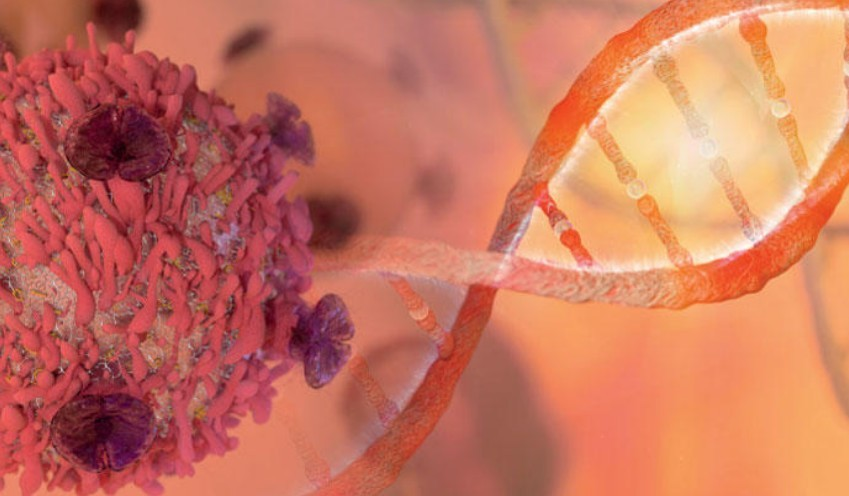
\includegraphics[width=\textwidth,height=0.6\textheight,keepaspectratio]{img/introduction/mot3.jpg}
		\label{img:mot2}
		\caption{Why a person has cancer?}
	\end{figure}
\end{frame}
%-------------------------------------------------------
%-------------------------------------------------------

%-------------------------------------------------------
%-------------------------------------------------------
\begin{frame}{The purpose of Bioinformatics}{Why some medicines no work in some persons?}
	\begin{figure}[]
		\centering
		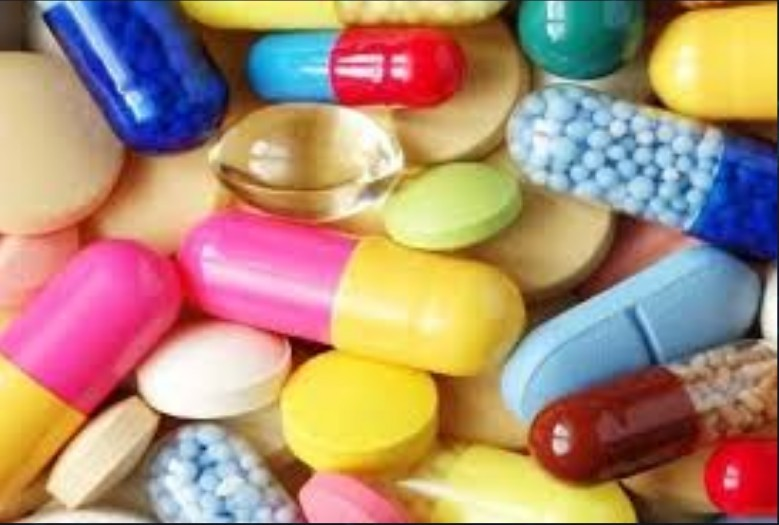
\includegraphics[width=\textwidth,height=0.6\textheight,keepaspectratio]{img/introduction/mot4.jpg}
		\label{img:mot2}
		\caption{Why some medicines no work in some persons?}
	\end{figure}
\end{frame}
%-------------------------------------------------------
%-------------------------------------------------------

%-------------------------------------------------------
%-------------------------------------------------------
\begin{frame}{The purpose of Bioinformatics}{Treatment Development}
	\begin{figure}[]
		\centering
		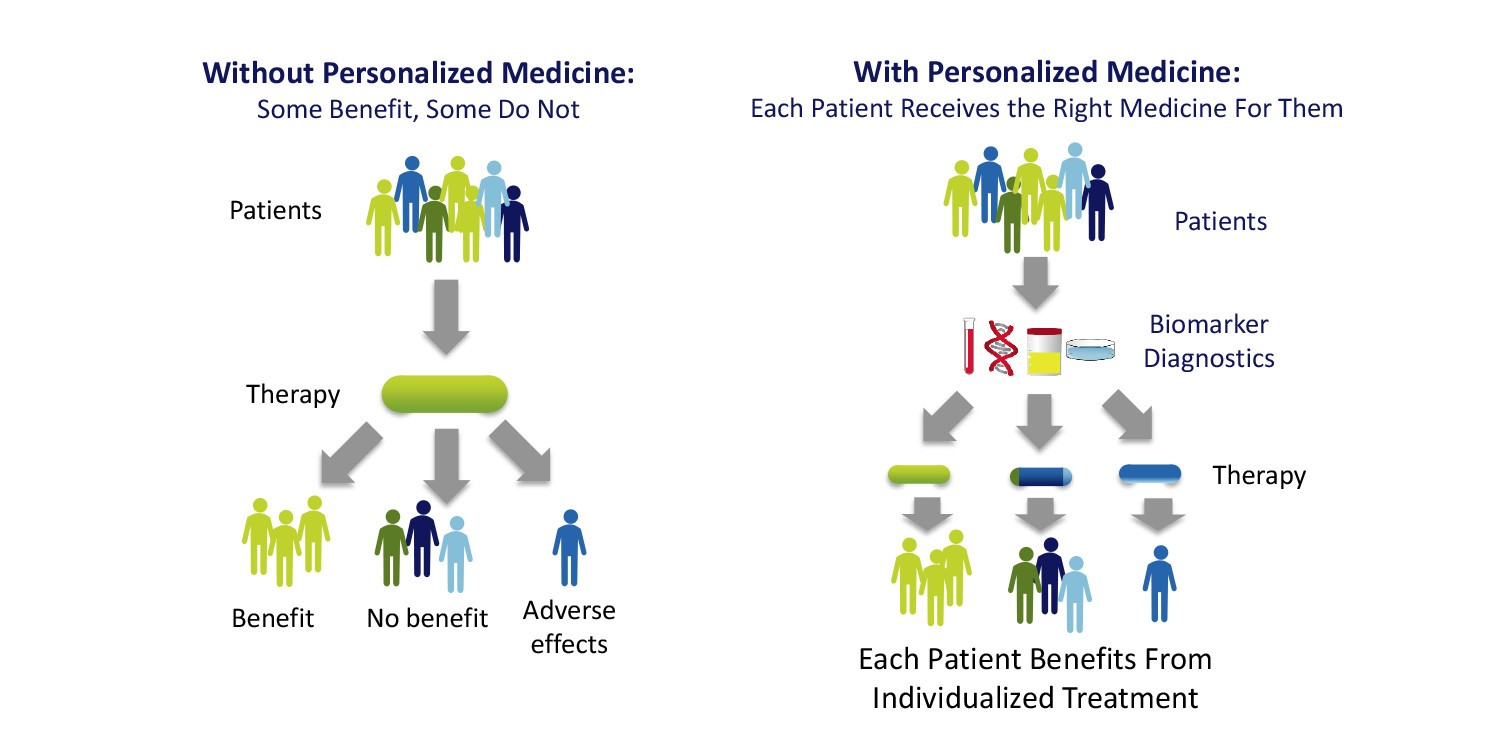
\includegraphics[width=\textwidth,height=0.7\textheight,keepaspectratio]{img/introduction/mot5.jpg}
		\label{img:mot2}
		\caption{Personalized Medicine: New Approach to Treatment of Disease}
	\end{figure}
\end{frame}
%-------------------------------------------------------
%-------------------------------------------------------

%-------------------------------------------------------
%-------------------------------------------------------
\begin{frame}{The purpose of Bioinformatics}{Protein structure prediction}
	\begin{figure}[]
		\centering
		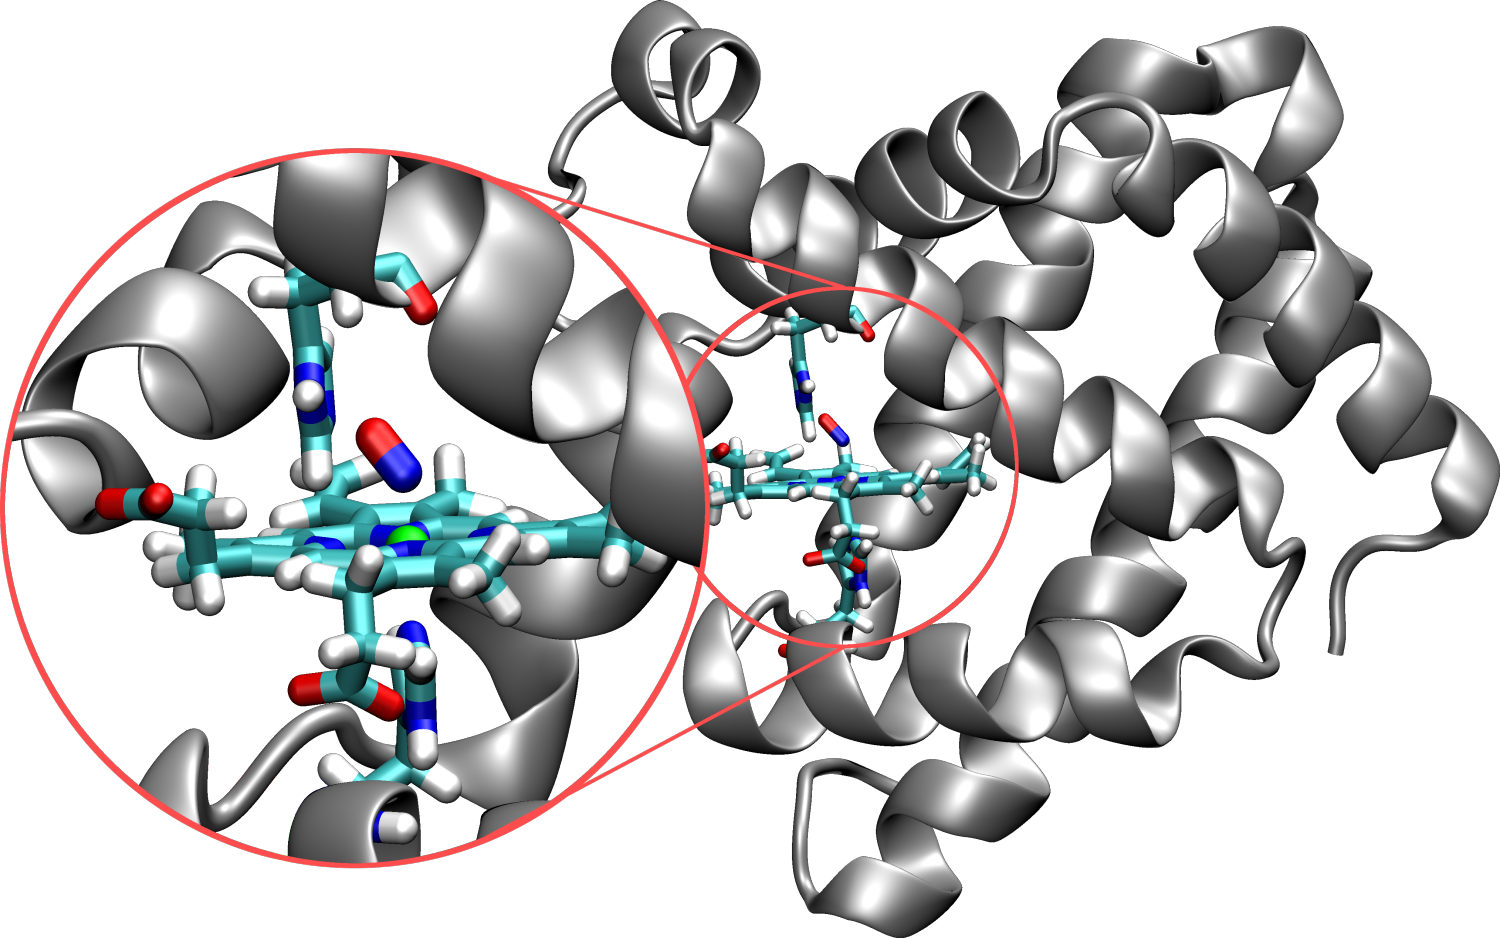
\includegraphics[width=\textwidth,height=0.7\textheight,keepaspectratio]{img/webinar/protein2}
		%https://www.pngwing.com/en/free-png-mrxlb
		\label{img:mot2}
		\caption{Computer simulation of protein-ligand.}
	\end{figure}
\end{frame}
%-------------------------------------------------------
%-------------------------------------------------------



%%%%%%%%%%%%%%%%%%%%%%%%%%%%%%%%%%%%%%%%%%%%%%%%%%%%%%%%
\subsection{What is Bioinformatics?}
%%%%%%%%%%%%%%%%%%%%%%%%%%%%%%%%%%%%%%%%%%%%%%%%%%%%%%%%

%-------------------------------------------------------
%-------------------------------------------------------
\begin{frame}{Introduction}{What is Bioinformatics?}
	
	According to Luscombe et al.: \textbf{Bioinformatics} involves the technology that uses computers for storage, retrieval, manipulation, and distribution of information related to biological macromolecules such as DNA, RNA, and proteins \cite{luscombe2001bioinformatics}.
	
\end{frame}
%-------------------------------------------------------
%-------------------------------------------------------


%-------------------------------------------------------
%-------------------------------------------------------
\begin{frame}{Bioinformatics}
	\begin{figure}[]
		\centering
		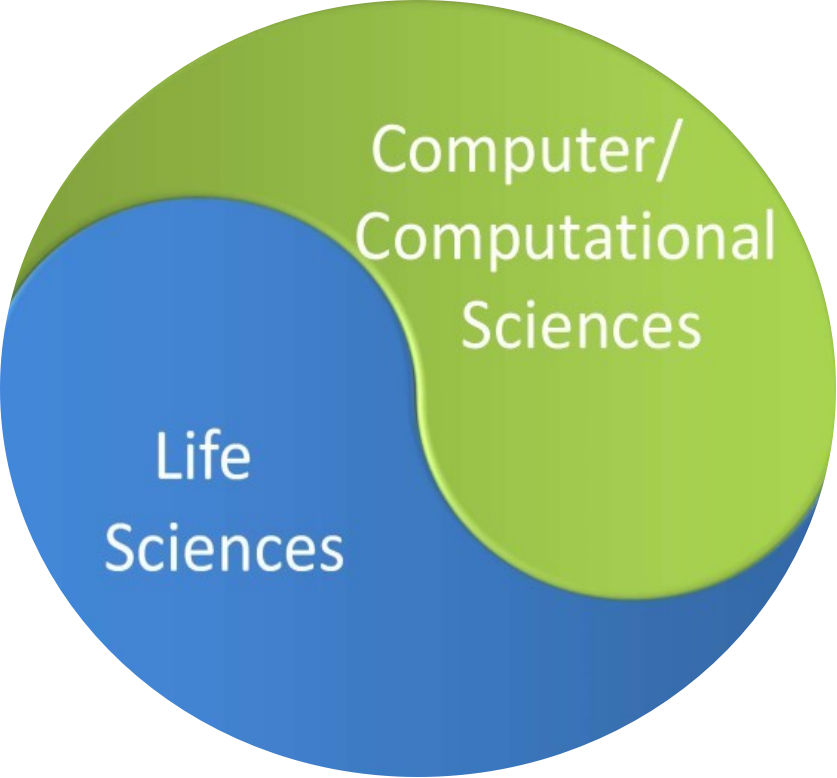
\includegraphics[width=\textwidth,height=0.7\textheight,keepaspectratio]{img/webinar/bio2.png}
		\label{img:mot2}
		%\caption{Computer simulation of protein-ligand.}
	\end{figure}
\end{frame}
%-------------------------------------------------------
%-------------------------------------------------------

%-------------------------------------------------------
%-------------------------------------------------------
\begin{frame}{Bioinformatics}
	\begin{figure}[]
		\centering
		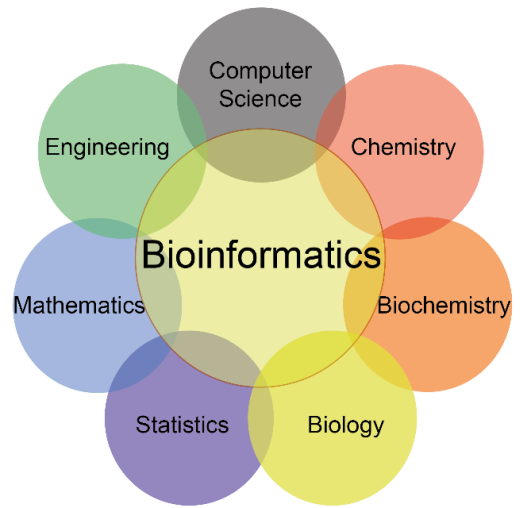
\includegraphics[width=\textwidth,height=0.7\textheight,keepaspectratio]{img/webinar/bio4}
		\label{img:mot2}
		%\caption{Computer simulation of protein-ligand.}
	\end{figure}
\end{frame}
%-------------------------------------------------------
%-------------------------------------------------------


%-------------------------------------------------------
%-------------------------------------------------------
\begin{frame}{Bioinformatics}{Concepts}
	\begin{figure}[]
		\centering
		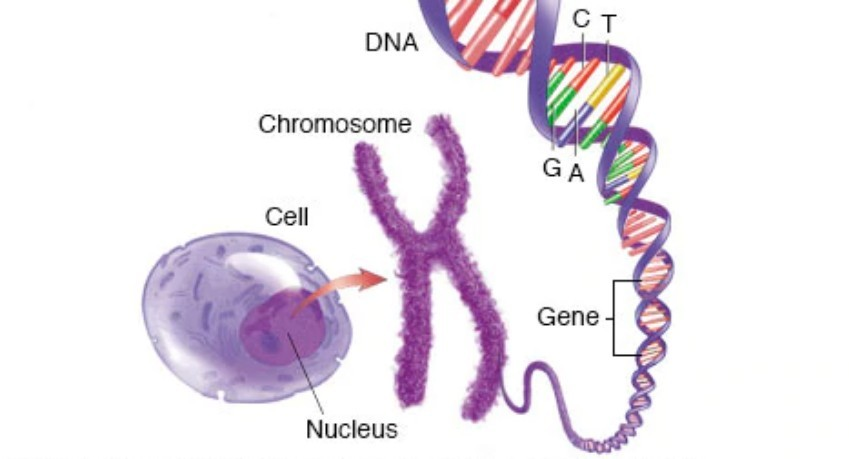
\includegraphics[width=\textwidth,height=0.6\textheight,keepaspectratio]{img/introduction/bio4.jpg}
		\label{img:mot2}
		\caption{Where DNA is located \cite{dna2020located}.}
	\end{figure}
\end{frame}
%-------------------------------------------------------
%-------------------------------------------------------

%-------------------------------------------------------
%-------------------------------------------------------
\begin{frame}{Bioinformatics}{Concepts}
	\begin{figure}[]
		\centering
		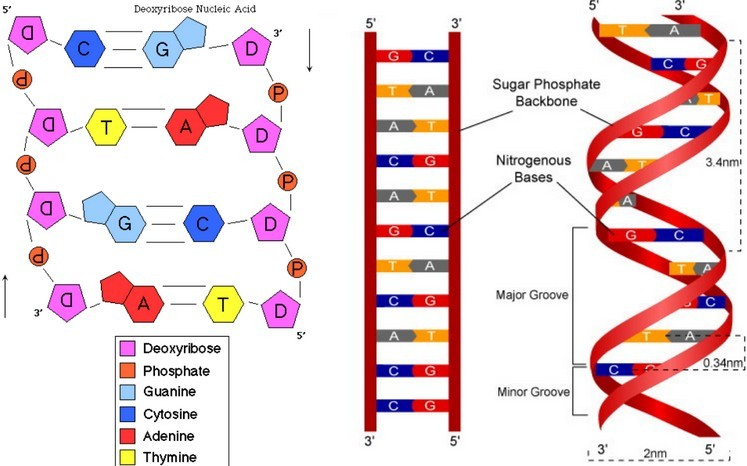
\includegraphics[width=\textwidth,height=0.7\textheight,keepaspectratio]{img/introduction/bio7.jpg}
		\label{img:mot2}
		\caption{DNA structure \cite{dnastructure2020}.}
	\end{figure}
\end{frame}
%-------------------------------------------------------
%-------------------------------------------------------



%-------------------------------------------------------
%-------------------------------------------------------
\begin{frame}{Bioinformatics}{Concepts}
	
	\begin{block}{}
		\centering
		The human genome is made of \textbf{\string ~3.2 billions bp} of DNA. \\
		\string ~6.4 billions of nucleotides \cite{archibald2018genomics}.
	\end{block}

	\pause
	\begin{block}{}
		\centering
		The HIV-1 genome is made of \textbf{\string ~20k bp} of DNA. \\
		Meanwhile, the COVID-19 is made of \textbf{\string ~32k bp} \cite{randhawa2020machine}.
	\end{block}

	\pause
	\begin{block}{}
		\centering
		There are approximately \textbf{19000} to \textbf{25000} genes. \\
		No one knows for sure \cite{archibald2018genomics}.
	\end{block}
	
\end{frame}
%-------------------------------------------------------
%-------------------------------------------------------

%-------------------------------------------------------
%-------------------------------------------------------
\begin{frame}{Bioinformatics}{Concepts}
	\begin{figure}[]
		\centering
		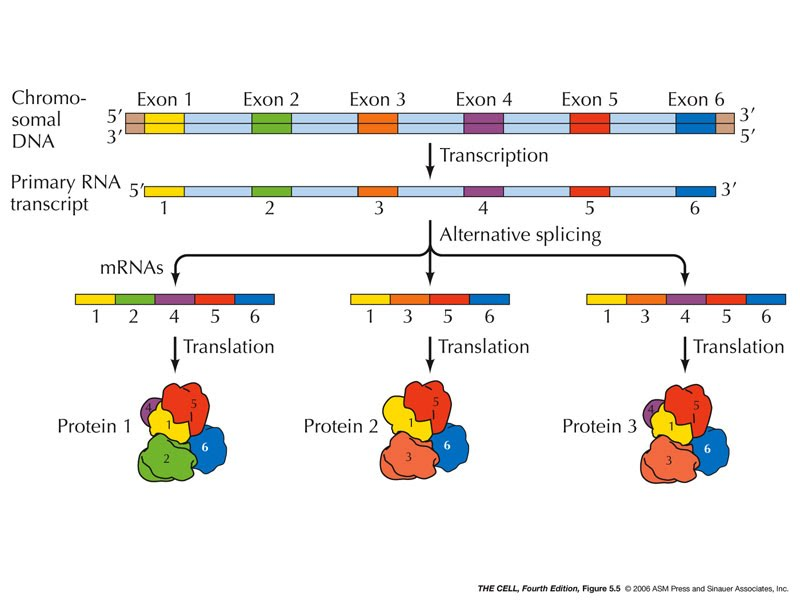
\includegraphics[width=\textwidth,height=0.7\textheight,keepaspectratio]{img/numbers/alt.jpg}
		\label{img:mot2}
		\caption{Alternative splicing \cite{genbio2020}.}
	\end{figure}
\end{frame}
%-------------------------------------------------------
%-------------------------------------------------------


%%%%%%%%%%%%%%%%%%%%%%%%%%%%%%%%%%%%%%%%%%%%%%%%%%%%%%%%%%%%%%%%%%%%%%%%%%%%%%%%%%%%%%%
%%%%%%%%%%%%%%%%%%%%%%%%%%%%%%%%%%%%%%%%%%%%%%%%%%%%%%%%%%%%%%%%%%%%%%%%%%%%%%%%%%%%%%%
\section{Bioinformatics against COVID-19}
%%%%%%%%%%%%%%%%%%%%%%%%%%%%%%%%%%%%%%%%%%%%%%%%%%%%%%%%%%%%%%%%%%%%%%%%%%%%%%%%%%%%%%%
%%%%%%%%%%%%%%%%%%%%%%%%%%%%%%%%%%%%%%%%%%%%%%%%%%%%%%%%%%%%%%%%%%%%%%%%%%%%%%%%%%%%%%%

%%%%%%%%%%%%%%%%%%%%%%%%%%%%%%%%%%%%%%%%%%%%%%%%%%%%%%%%%%%%%%%%%%%%%%%%%%%%%%%%%%%%%%%
%%%%%%%%%%%%%%%%%%%%%%%%%%%%%%%%%%%%%%%%%%%%%%%%%%%%%%%%%%%%%%%%%%%%%%%%%%%%%%%%%%%%%%%
%\subsection{COVID-19}
%%%%%%%%%%%%%%%%%%%%%%%%%%%%%%%%%%%%%%%%%%%%%%%%%%%%%%%%%%%%%%%%%%%%%%%%%%%%%%%%%%%%%%%
%%%%%%%%%%%%%%%%%%%%%%%%%%%%%%%%%%%%%%%%%%%%%%%%%%%%%%%%%%%%%%%%%%%%%%%%%%%%%%%%%%%%%%%

%-------------------------------------------------------
%-------------------------------------------------------
%\begin{frame}{COVID-19}
%	\begin{figure}[]
%		\centering
%		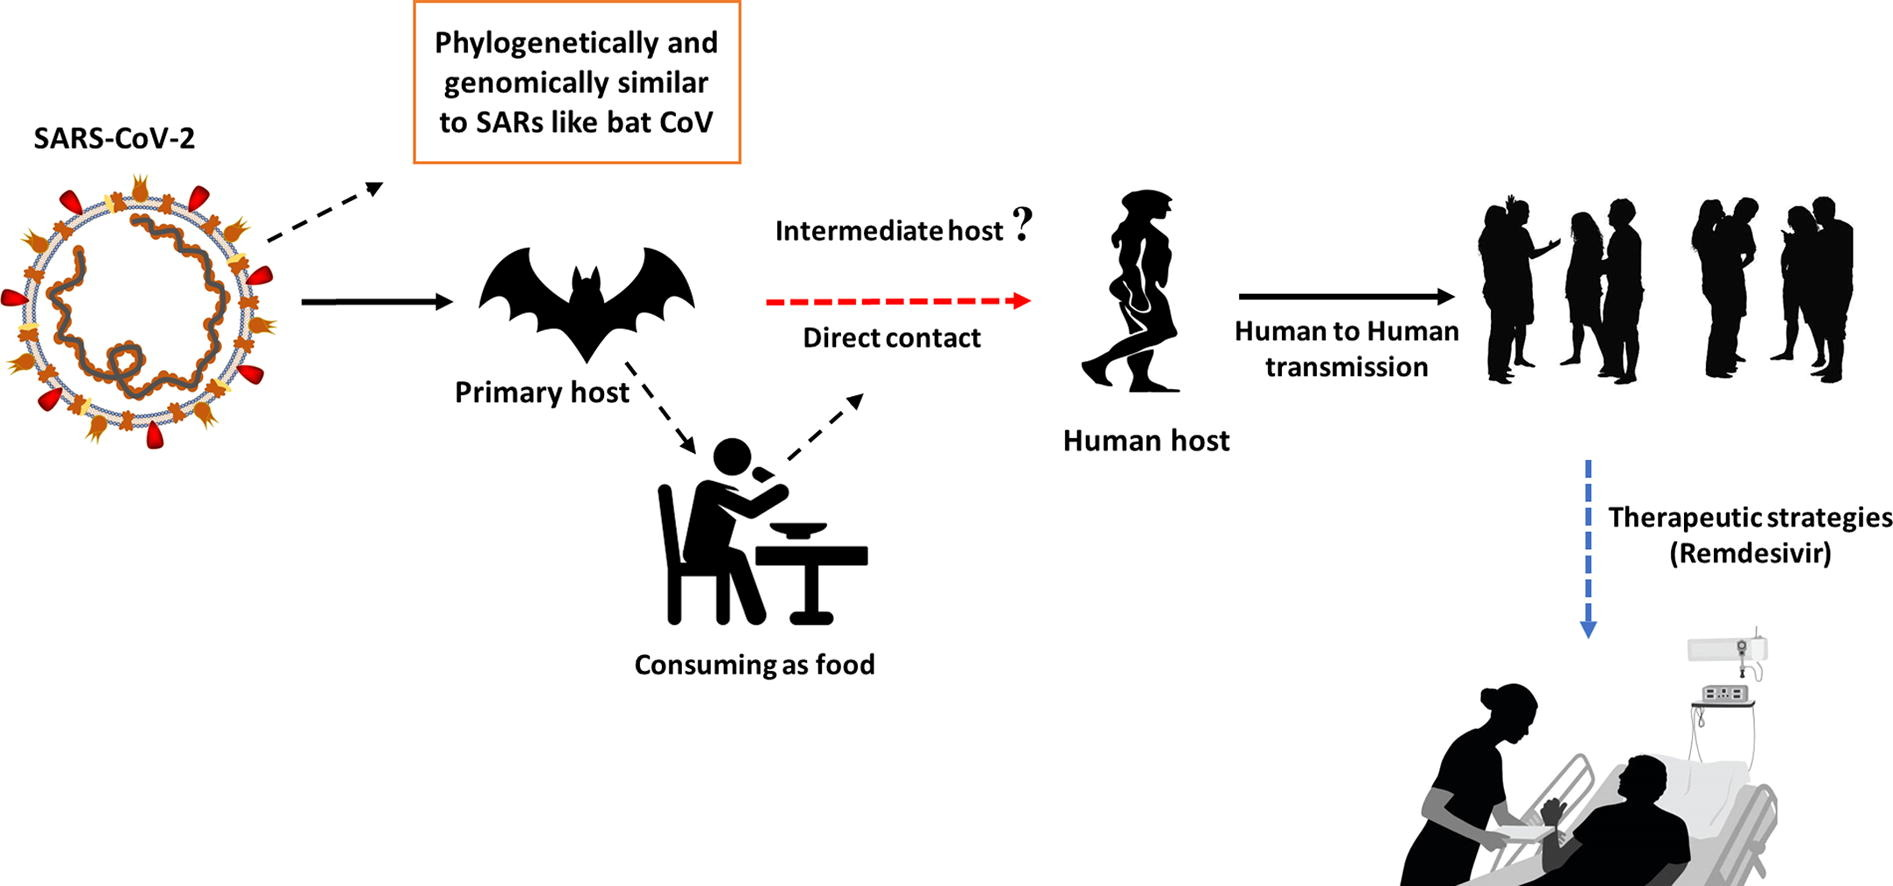
\includegraphics[width=\textwidth,keepaspectratio]{img/webinar/covid_origin}
%		\label{img:mot2}
%		\caption{Graphical origin of COVID-19. Source: \cite{shereen2020covid}}
%	\end{figure}
%\end{frame}
%-------------------------------------------------------
%-------------------------------------------------------


%%%%%%%%%%%%%%%%%%%%%%%%%%%%%%%%%%%%%%%%%%%%%%%%%%%%%%%%%%%%%%%%%%%%%%%%%%%%%%%%%%%%%%%
%%%%%%%%%%%%%%%%%%%%%%%%%%%%%%%%%%%%%%%%%%%%%%%%%%%%%%%%%%%%%%%%%%%%%%%%%%%%%%%%%%%%%%%
\subsection{COVID origin}
%%%%%%%%%%%%%%%%%%%%%%%%%%%%%%%%%%%%%%%%%%%%%%%%%%%%%%%%%%%%%%%%%%%%%%%%%%%%%%%%%%%%%%%
%%%%%%%%%%%%%%%%%%%%%%%%%%%%%%%%%%%%%%%%%%%%%%%%%%%%%%%%%%%%%%%%%%%%%%%%%%%%%%%%%%%%%%%

%-------------------------------------------------------
%-------------------------------------------------------
\begin{frame}{COVID origin}{Phylogenetic tree and BLAST}
	\begin{figure}[]
		\centering
		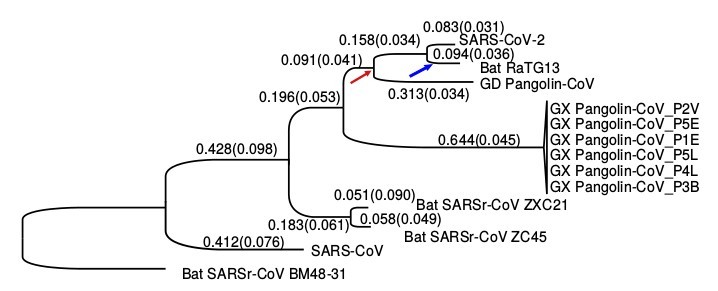
\includegraphics[width=\textwidth,height=0.7\textheight,keepaspectratio]{img/alignment/phylocovid.jpg}
		\label{img:mot2}
		\caption{The phylogenetic tree of SARS-CoV-2 (COVID-19) and the related Coronaviruses  \cite{tang2020origin}.}
	\end{figure}
\end{frame}
%-------------------------------------------------------
%-------------------------------------------------------

%-------------------------------------------------------
%-------------------------------------------------------
\begin{frame}{COVID origin}{Novel virus classification using alignment-free methods}
	\begin{figure}[]
		\centering
		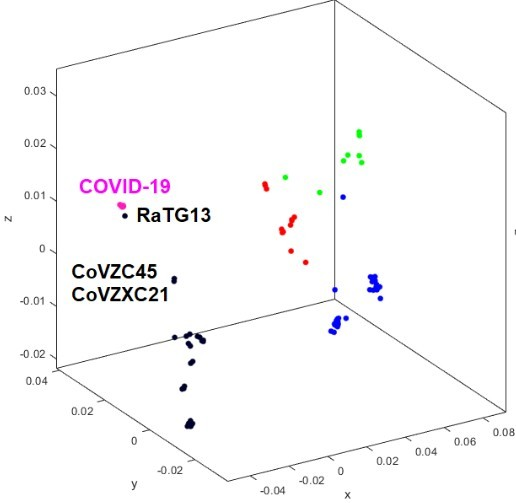
\includegraphics[width=\textwidth,height=0.7\textheight,keepaspectratio]{img/webinar/modmap3d}
		\label{img:mot2}
		\caption{MoDMap3D of 124 Betacoronavirus sequences and COVID-19 \cite{randhawa2020machine}.}
	\end{figure}
\end{frame}
%-------------------------------------------------------
%-------------------------------------------------------


%%%%%%%%%%%%%%%%%%%%%%%%%%%%%%%%%%%%%%%%%%%%%%%%%%%%%%%%%%%%%%%%%%%%%%%%%%%%%%%%%%%%%%%
%%%%%%%%%%%%%%%%%%%%%%%%%%%%%%%%%%%%%%%%%%%%%%%%%%%%%%%%%%%%%%%%%%%%%%%%%%%%%%%%%%%%%%%
\subsection{Protein structure prediction}
%%%%%%%%%%%%%%%%%%%%%%%%%%%%%%%%%%%%%%%%%%%%%%%%%%%%%%%%%%%%%%%%%%%%%%%%%%%%%%%%%%%%%%%
%%%%%%%%%%%%%%%%%%%%%%%%%%%%%%%%%%%%%%%%%%%%%%%%%%%%%%%%%%%%%%%%%%%%%%%%%%%%%%%%%%%%%%%

%-------------------------------------------------------
%-------------------------------------------------------
\begin{frame}{Protein structure prediction}{Definition}
	\begin{block}{Definition}
		The prediction of protein three-dimensional structure from amino acid sequence \cite{kuhlman2019advances}.
	\end{block}

	\pause
	\begin{block}{Methods}
		\begin{itemize}
			\item X-ray crystallography.
			\item Nuclear magnetic resonance.
			\item Cryo-electron microscopy.
		\end{itemize}
	\end{block}
\end{frame}
%-------------------------------------------------------
%-------------------------------------------------------

%-------------------------------------------------------
%-------------------------------------------------------
\begin{frame}{Protein structure prediction}{Using computers}
	\begin{block}{}
		There are two aproaches to predicting protein structures:
		\begin{itemize}
			\item Homology modeling.
			\item Physical modeling.
		\end{itemize}
	\end{block}
	
\end{frame}
%-------------------------------------------------------
%-------------------------------------------------------

%-------------------------------------------------------
%-------------------------------------------------------
\begin{frame}{Protein structure prediction}{Proteins in COVID-19}
	\begin{figure}[]
		\centering
		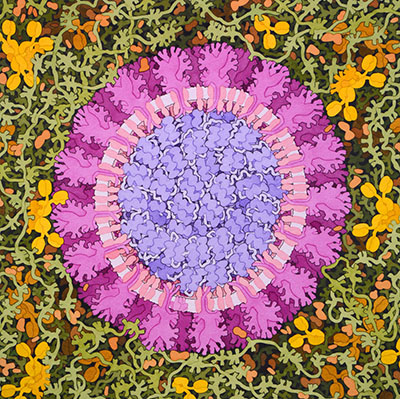
\includegraphics[width=0.5\textwidth,keepaspectratio]{img/webinar/covid}
		\label{img:mot2}
		\caption{Graphical view of COVID-19 structure. Source: \cite{Goodsell2020}}
	\end{figure}
\end{frame}
%-------------------------------------------------------
%-------------------------------------------------------

%-------------------------------------------------------
%-------------------------------------------------------
\begin{frame}{Protein structure prediction}{Proteins in COVID-19}
	\begin{figure}[]
		\centering
		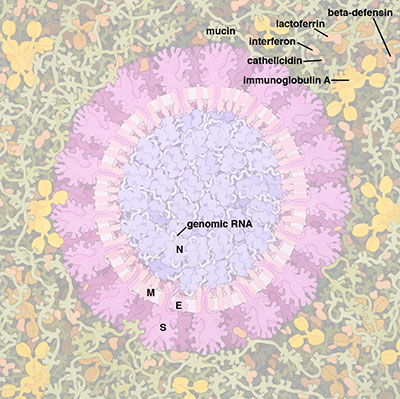
\includegraphics[width=0.5\textwidth,keepaspectratio]{img/webinar/covid2}
		\label{img:mot2}
		\caption{Membrane S (spike) protein, M (membrane) protein, membrane channel E (envelope) protein and the N (nucleocapsid) protein bound to the genomic RNA. Source: \cite{Goodsell2020}}
	\end{figure}
\end{frame}
%-------------------------------------------------------
%-------------------------------------------------------


%-------------------------------------------------------
%-------------------------------------------------------
\begin{frame}{Protein structure prediction}{AlphaFold method}
	\begin{figure}[]
		\centering
		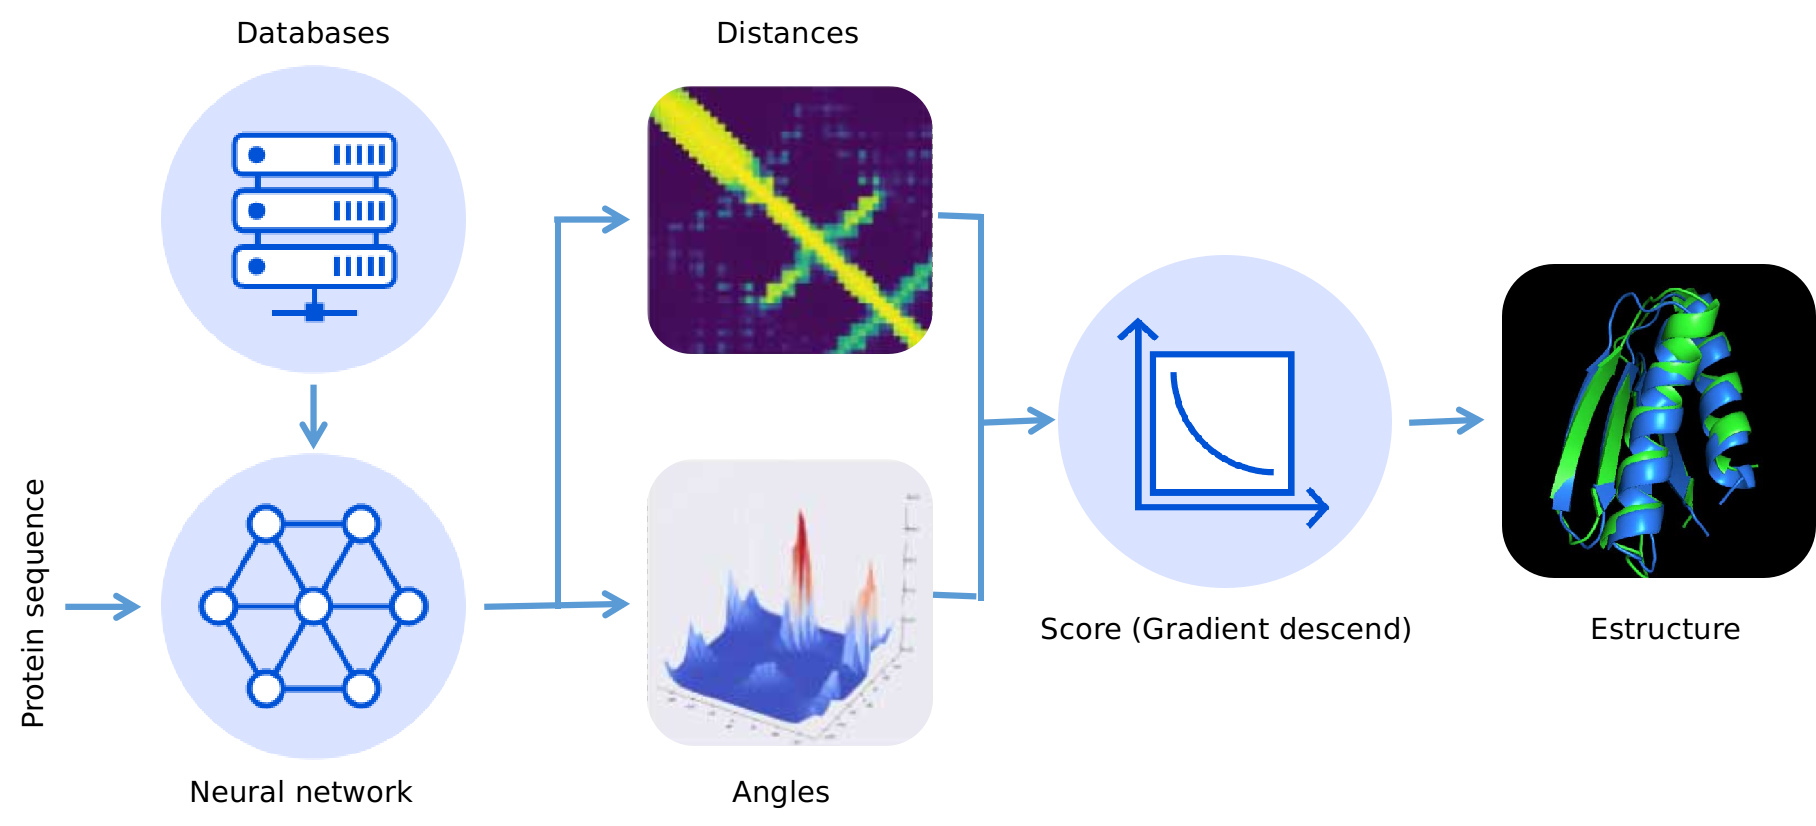
\includegraphics[width=\textwidth,keepaspectratio]{img/webinar/protein_prediction}
		\label{img:mot2}
		\caption{Protein structure prediction method proposed by AlphaFold. Source: \cite{alphafold2020}}
	\end{figure}
\end{frame}
%-------------------------------------------------------
%-------------------------------------------------------

%-------------------------------------------------------
%-------------------------------------------------------
\begin{frame}{Protein structure prediction}{COVID-19 membrane protein}
	\begin{figure}[]
		\centering
		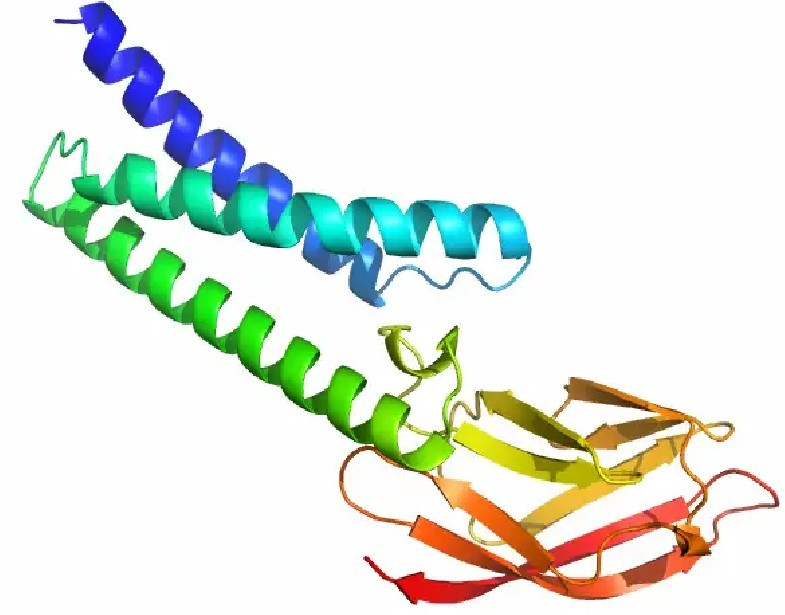
\includegraphics[width=0.7\textwidth,keepaspectratio]{img/webinar/covid3}
		\label{img:mot2}
		\caption{COVID-19 membrane protein. Source: \cite{alphafold2020}}
	\end{figure}
\end{frame}
%-------------------------------------------------------
%-------------------------------------------------------


%-------------------------------------------------------
%-------------------------------------------------------
\begin{frame}{Protein structure prediction}{Tertiary representations of the S1 and S2 subunits of the spike protein}
	\begin{figure}[]
		\centering
		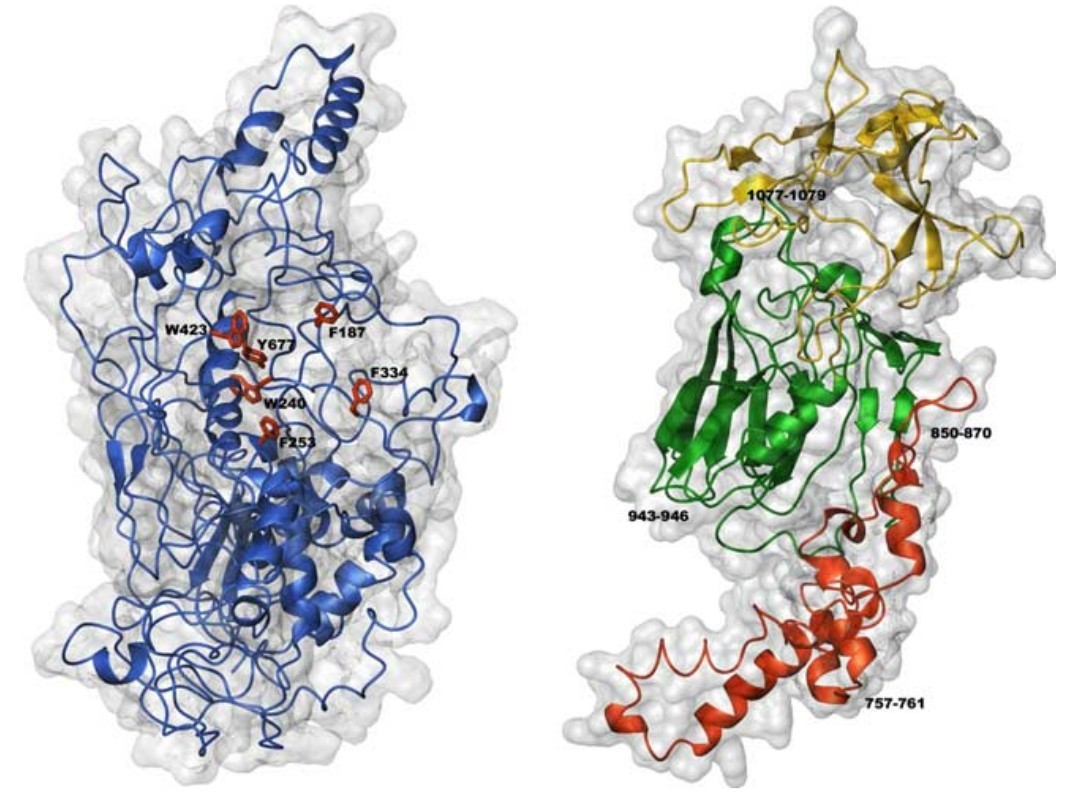
\includegraphics[width=0.7\textwidth,keepaspectratio]{img/webinar/s1s2}
		\label{img:mot2}
		\caption{Tertiary representations of the S1 and S2 subunits of the spike protein using PsiPred. Source: \cite{spiga2003molecular}}
	\end{figure}
\end{frame}
%-------------------------------------------------------
%-------------------------------------------------------




%%%%%%%%%%%%%%%%%%%%%%%%%%%%%%%%%%%%%%%%%%%%%%%%%%%%%%%%%%%%%%%%%%%%%%%%%%%%%%%%%%%%%%%
%%%%%%%%%%%%%%%%%%%%%%%%%%%%%%%%%%%%%%%%%%%%%%%%%%%%%%%%%%%%%%%%%%%%%%%%%%%%%%%%%%%%%%%
\subsection{Drug discovery}
%%%%%%%%%%%%%%%%%%%%%%%%%%%%%%%%%%%%%%%%%%%%%%%%%%%%%%%%%%%%%%%%%%%%%%%%%%%%%%%%%%%%%%%
%%%%%%%%%%%%%%%%%%%%%%%%%%%%%%%%%%%%%%%%%%%%%%%%%%%%%%%%%%%%%%%%%%%%%%%%%%%%%%%%%%%%%%%

%-------------------------------------------------------
%-------------------------------------------------------
\begin{frame}{Drug discovery}{Definition}
	\begin{block}{Definition}
		Drug discovery is the process by new candidate medications are discovered \cite{usafooddrug2020}.
	\end{block}
\end{frame}
%-------------------------------------------------------
%-------------------------------------------------------


%-------------------------------------------------------
%-------------------------------------------------------
\begin{frame}{Drug discovery}{From a million to one}
	\begin{figure}[]
		\centering
		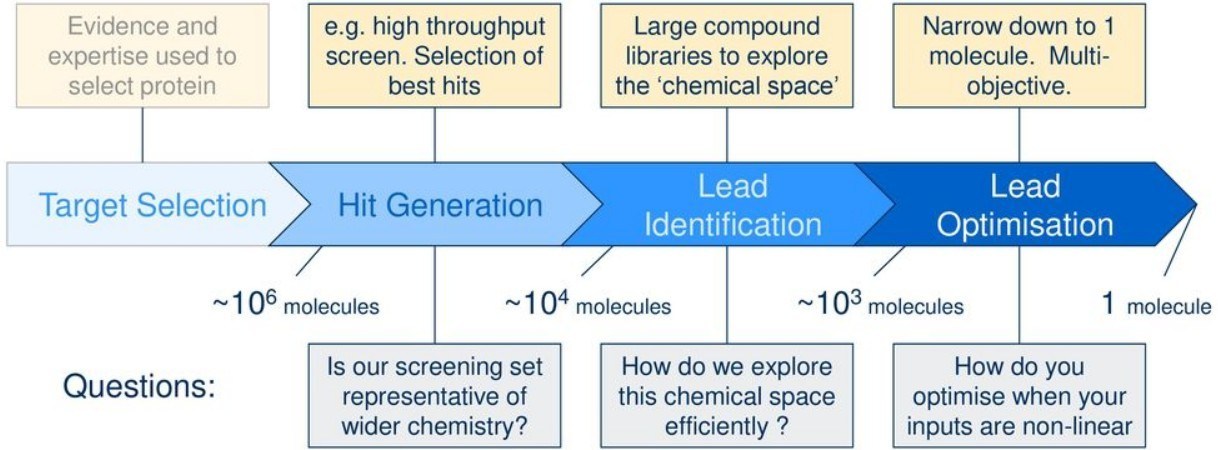
\includegraphics[width=\textwidth,keepaspectratio]{img/webinar/drug2}
		\label{img:mot2}
		\caption{Process in drug discovery. Source: \cite{chanin2020}}
	\end{figure}
\end{frame}
%-------------------------------------------------------
%-------------------------------------------------------

%-------------------------------------------------------
%-------------------------------------------------------
\begin{frame}{Drug discovery}{COVID-19 main protease}
	\begin{figure}[]
		\centering
		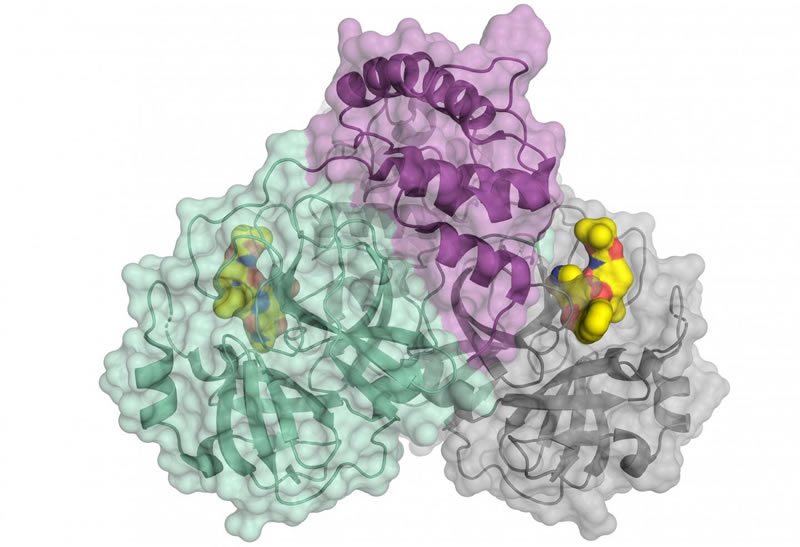
\includegraphics[width=0.8\textwidth,keepaspectratio]{img/webinar/protease}
		\label{img:mot2}
		\caption{Schematic representation of the coronavirus protease. Source: \cite{zhang2020crystal}}
	\end{figure}
\end{frame}
%-------------------------------------------------------
%-------------------------------------------------------



%-------------------------------------------------------
%-------------------------------------------------------
\begin{frame}{Drug discovery}{N3 inhibitor of main protease}
	\begin{figure}[]
		\centering
		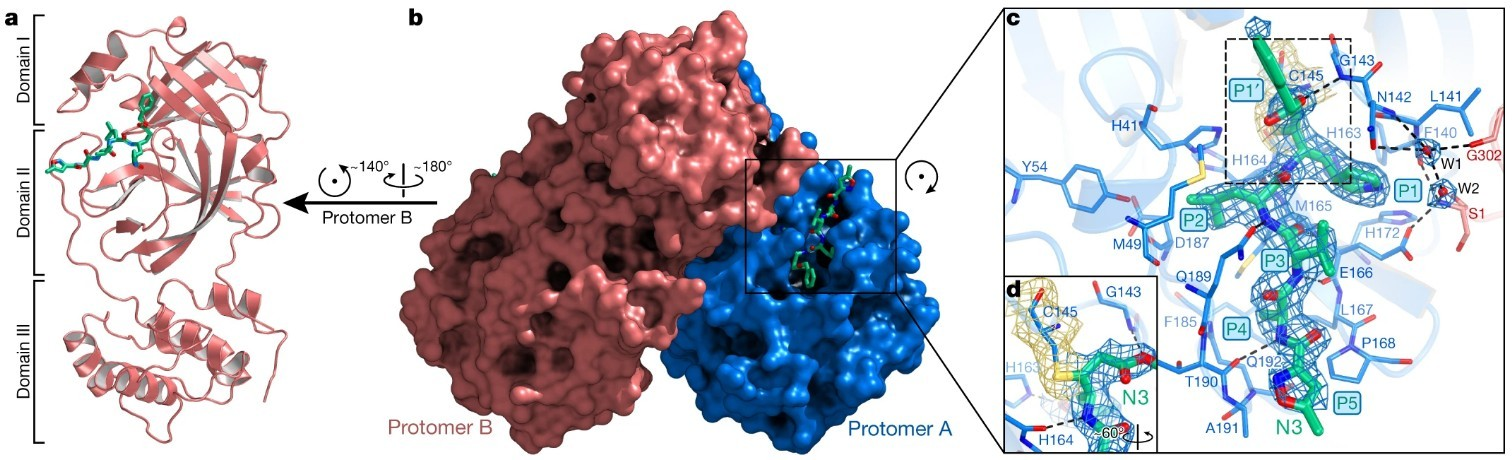
\includegraphics[width=\textwidth,keepaspectratio]{img/webinar/drug}
		\label{img:mot2}
		\caption{The crystal structure of SARS-CoV-2 main protease N3 inhibitor. Source: \cite{jin2020structure}}
	\end{figure}
\end{frame}
%-------------------------------------------------------
%-------------------------------------------------------

%-------------------------------------------------------
%-------------------------------------------------------
\begin{frame}{Drug discovery}{Molecular docking with Glide}
	\begin{figure}[]
		\centering
		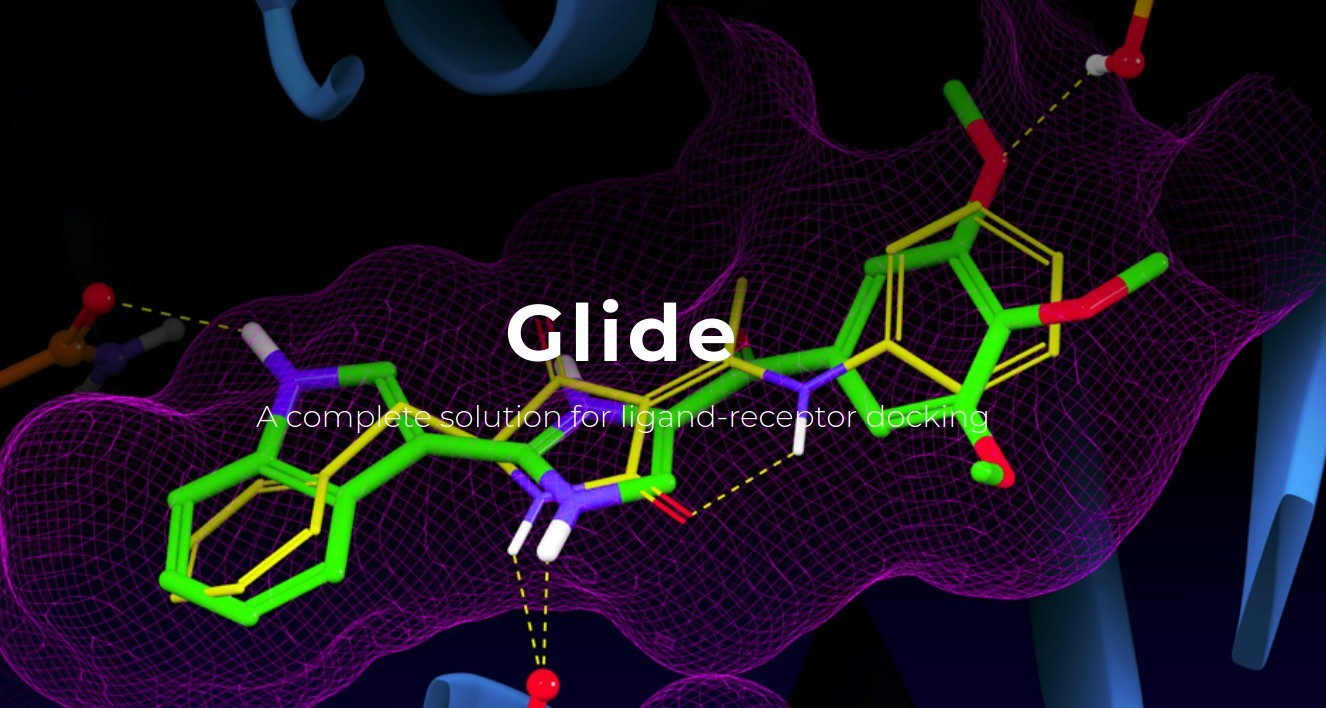
\includegraphics[width=\textwidth,keepaspectratio]{img/webinar/glide}
		\label{img:mot2}
		%\caption{Glide offers the full range of speed vs. accuracy options, from the HTVS (high-throughput virtual screening) mode for efficiently enriching million compound libraries, to the SP (standard precision) mode for reliably docking tens to hundreds of thousands of ligand with high accuracy.}
	\end{figure}
\end{frame}
%-------------------------------------------------------
%-------------------------------------------------------

%-------------------------------------------------------
%-------------------------------------------------------
\begin{frame}{Drug discovery}{Molecular docking}
	\begin{block}{Molecular docking}
		Molecular docking is a computer simulation procedure to
		predict the conformation of a receptor-ligand complex \cite{dias2008molecular}
	\end{block}

	\begin{block}{}
		Algorithms used:
		\begin{itemize}
			\item Fast shape matching (take into account the geometric).
			\item Simulated Anneling.
			\item Genetic algorithms.
			\item Tabu search.
		\end{itemize}
	\end{block}
\end{frame}
%-------------------------------------------------------
%-------------------------------------------------------



%-------------------------------------------------------
%-------------------------------------------------------
\begin{frame}{Drug discovery}{Protease Inhibitors Designed Using Generative Deep Learning Approaches}
	\begin{figure}[]
		\centering
		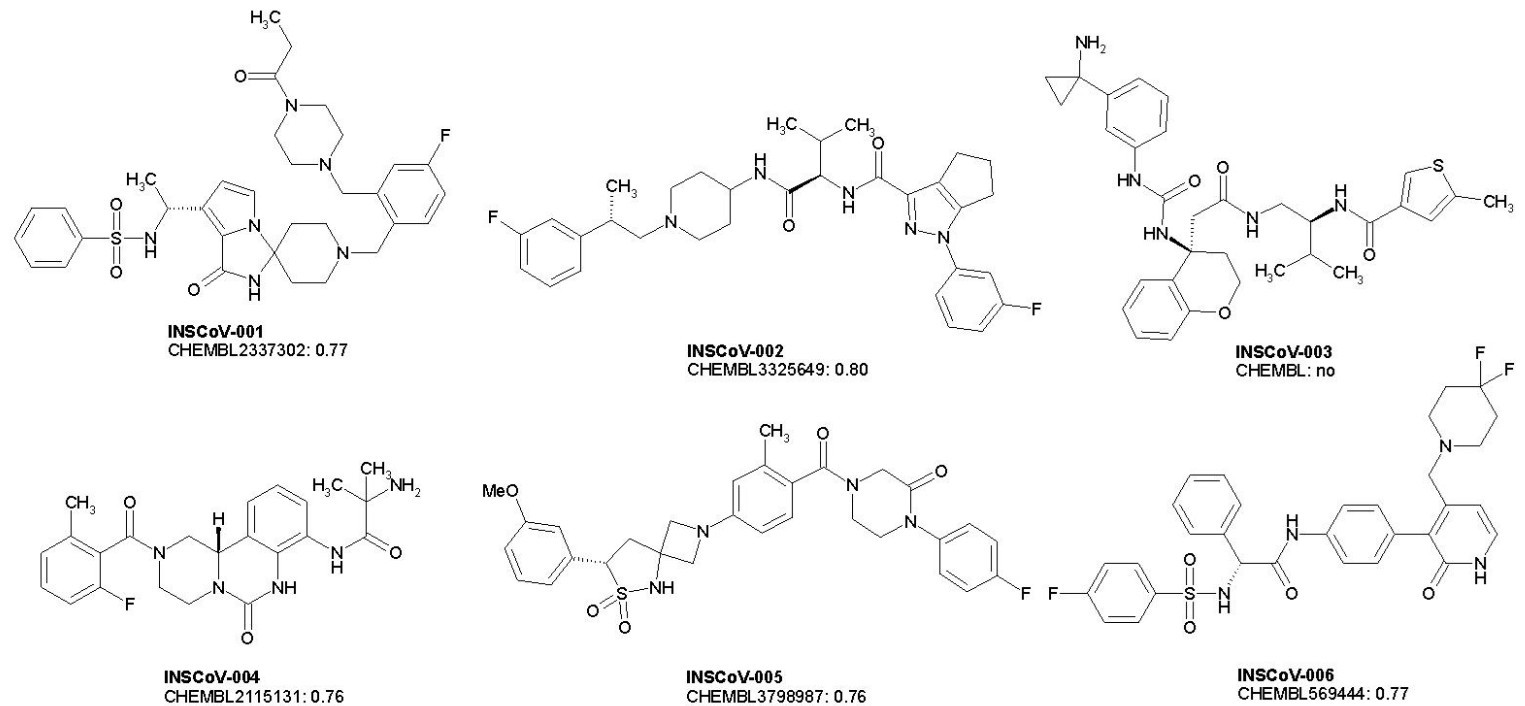
\includegraphics[width=\textwidth,keepaspectratio]{img/webinar/drug3}
		\label{img:mot2}
		\caption{Representative examples of the structures generated to target the main protease of
			2019-nCoV. Novelty was assessed using similarity search in ChEMBL Database. Source: \cite{Zhavoronkov2020}}
	\end{figure}
\end{frame}
%-------------------------------------------------------
%-------------------------------------------------------



%%%%%%%%%%%%%%%%%%%%%%%%%%%%%%%%%%%%%%%%%%%%%%%%%%%%%%%%%%%%%%%%%%%%%%%%%%%%%%%%%%%%%%%
%%%%%%%%%%%%%%%%%%%%%%%%%%%%%%%%%%%%%%%%%%%%%%%%%%%%%%%%%%%%%%%%%%%%%%%%%%%%%%%%%%%%%%%
\subsection{Funding}
%%%%%%%%%%%%%%%%%%%%%%%%%%%%%%%%%%%%%%%%%%%%%%%%%%%%%%%%%%%%%%%%%%%%%%%%%%%%%%%%%%%%%%%
%%%%%%%%%%%%%%%%%%%%%%%%%%%%%%%%%%%%%%%%%%%%%%%%%%%%%%%%%%%%%%%%%%%%%%%%%%%%%%%%%%%%%%%


%-------------------------------------------------------
%-------------------------------------------------------
\begin{frame}{Funding}{Coronavirus Funding Monitor}
	List of open funding calls and other support for researchers, non-profit organizations and commercial organizations, specifically for COVID-19 and coronavirus-related research (\href{https://coronavirus.frontiersin.org/covid-19-research-funding-monitor?utm_source=ad&utm_medium=lk&utm_campaign=ba_cov-cco_corp}{\color{blue}{\underline{Link}}}).
	\begin{figure}[]
		\centering
		
\includegraphics[width=\textwidth,keepaspectratio]{img/webinar/res1}				
	\end{figure}

	\begin{figure}[]
		\centering
		
\includegraphics[width=0.5\textwidth,keepaspectratio]{img/webinar/res2}				
	\end{figure}
\end{frame}
%-------------------------------------------------------
%-------------------------------------------------------

%-------------------------------------------------------
%-------------------------------------------------------
\begin{frame}{Funding}{MIT CVID-19 challenges }
	MIT is hosting a series of challenges to empower YOU to take action on the COVID-19 crisis (\href{https://covid19challenge.mit.edu/}{\color{blue}{\underline{Link}}}).
	\begin{figure}[]
		\centering
		
\includegraphics[width=\textwidth,keepaspectratio]{img/webinar/res3}				
	\end{figure}	
\end{frame}
%-------------------------------------------------------
%-------------------------------------------------------

%-------------------------------------------------------
%-------------------------------------------------------
\begin{frame}{Funding}{FONDECYT}	
	\begin{figure}[]
		\centering
		
\includegraphics[width=\textwidth,keepaspectratio]{img/webinar/res7}				
	\end{figure}	
\end{frame}
%-------------------------------------------------------
%-------------------------------------------------------

%%%%%%%%%%%%%%%%%%%%%%%%%%%%%%%%%%%%%%%%%%%%%%%%%%%%%%%%%%%%%%%%%%%%%%%%%%%%%%%%%%%%%%%
%%%%%%%%%%%%%%%%%%%%%%%%%%%%%%%%%%%%%%%%%%%%%%%%%%%%%%%%%%%%%%%%%%%%%%%%%%%%%%%%%%%%%%%
\subsection{Datasets and resources}
%%%%%%%%%%%%%%%%%%%%%%%%%%%%%%%%%%%%%%%%%%%%%%%%%%%%%%%%%%%%%%%%%%%%%%%%%%%%%%%%%%%%%%%
%%%%%%%%%%%%%%%%%%%%%%%%%%%%%%%%%%%%%%%%%%%%%%%%%%%%%%%%%%%%%%%%%%%%%%%%%%%%%%%%%%%%%%%

%-------------------------------------------------------
%-------------------------------------------------------
\begin{frame}{Datasets and resources}{Coronavirus updates}
	Links to bioinformatics resources useful to track the evolution and progression as well as to manage genomics data (\href{http://www.clinbioinfosspa.es/CovidResources}{\color{blue}{\underline{Link}}}).
	\begin{figure}[]
		\centering
		
\includegraphics[width=\textwidth,keepaspectratio]{img/webinar/res4}				
	\end{figure}	
\end{frame}
%-------------------------------------------------------
%-------------------------------------------------------


%-------------------------------------------------------
%-------------------------------------------------------
\begin{frame}{Datasets and resources}{Institut Français de Bioinformatique (IFB)}
	The IFB offers expertise and computing facilities to support the involved teams on COVID-19 (\href{https://www.france-bioinformatique.fr/en/action-covid-19}{\color{blue}{\underline{Link}}}).
	\begin{figure}[]
		\centering
		
\includegraphics[width=0.7\textwidth,keepaspectratio]{img/webinar/res5}				
	\end{figure}	
\end{frame}
%-------------------------------------------------------
%-------------------------------------------------------

%-------------------------------------------------------
%-------------------------------------------------------
\begin{frame}{Datasets and resources}{The European Bioinformatics Institute (EMBL-EBI)}
	EMBL-EBI is gathering and sharing data resources as they become available (\href{https://www.ebi.ac.uk/about/news/announcements/coronavirus-data}{\color{blue}{\underline{Link}}}).
	\begin{figure}[]
		\centering
		
\includegraphics[width=0.8\textwidth,keepaspectratio]{img/webinar/res6.jpg}				
	\end{figure}	
\end{frame}
%-------------------------------------------------------
%-------------------------------------------------------


%%%%%%%%%%%%%%%%%%%%%%%%%%%%%%%%%%%%%%%%%%%%%%%%%%%%%%%%%%%%%%%%%%%%%%%%%%%%%%%%%%%%%%%
%%%%%%%%%%%%%%%%%%%%%%%%%%%%%%%%%%%%%%%%%%%%%%%%%%%%%%%%%%%%%%%%%%%%%%%%%%%%%%%%%%%%%%%
\section{How to learn?}
%%%%%%%%%%%%%%%%%%%%%%%%%%%%%%%%%%%%%%%%%%%%%%%%%%%%%%%%%%%%%%%%%%%%%%%%%%%%%%%%%%%%%%%
%%%%%%%%%%%%%%%%%%%%%%%%%%%%%%%%%%%%%%%%%%%%%%%%%%%%%%%%%%%%%%%%%%%%%%%%%%%%%%%%%%%%%%%

%%%%%%%%%%%%%%%%%%%%%%%%%%%%%%%%%%%%%%%%%%%%%%%%%%%%%%%%%%%%%%%%%%%%%%%%%%%%%%%%%%%%%%%
%%%%%%%%%%%%%%%%%%%%%%%%%%%%%%%%%%%%%%%%%%%%%%%%%%%%%%%%%%%%%%%%%%%%%%%%%%%%%%%%%%%%%%%
\subsection{How to learn Bioinformatics?}
%%%%%%%%%%%%%%%%%%%%%%%%%%%%%%%%%%%%%%%%%%%%%%%%%%%%%%%%%%%%%%%%%%%%%%%%%%%%%%%%%%%%%%%
%%%%%%%%%%%%%%%%%%%%%%%%%%%%%%%%%%%%%%%%%%%%%%%%%%%%%%%%%%%%%%%%%%%%%%%%%%%%%%%%%%%%%%%

%-------------------------------------------------------
%-------------------------------------------------------
\begin{frame}{How to learn Bioinformatics?}{Biology as a DATA SCIENCE}
	T-Bio platform (\href{https://edu.t-bio.info/}{\color{blue}{\underline{Link}}}).
	\begin{figure}[]
		\centering
		
\includegraphics[width=\textwidth,keepaspectratio]{img/webinar/tbio.jpg}				
	\end{figure}	
\end{frame}
%-------------------------------------------------------
%-------------------------------------------------------

%-------------------------------------------------------
%-------------------------------------------------------
\begin{frame}{How to learn Bioinformatics?}{Coursera}
	Coursera (\href{https://www.coursera.org/}{\color{blue}{\underline{Link}}}).
	\begin{figure}[]
		\centering
		
\includegraphics[width=0.8\textwidth,keepaspectratio]{img/webinar/coursera.jpg}				
	\end{figure}	
\end{frame}
%-------------------------------------------------------
%-------------------------------------------------------

%-------------------------------------------------------
%-------------------------------------------------------
\begin{frame}{How to learn Bioinformatics?}{Bioinformatics Research Group}
	Bioinformatics Research Group at la Salle university is a interdisciplinary group open for everybody who have a computer science` background. 
	\begin{figure}[]
		\centering
		
\includegraphics[width=0.3\textwidth,keepaspectratio]{img/webinar/salle}				
	\end{figure}	
\end{frame}
%-------------------------------------------------------
%-------------------------------------------------------




%-------------------------------------------------------
%-------------------------------------------------------
\begin{frame}[allowframebreaks]
	\frametitle{References}
	%\bibliographystyle{amsalpha}
	\bibliographystyle{IEEEtran}
	\bibliography{bibliography}
\end{frame}
%-------------------------------------------------------
%-------------------------------------------------------



%-------------------------------------------------------
%-------------------------------------------------------
\if\mycmd1 % MY THEME
\1{
	{\1
		\begin{frame}[plain,noframenumbering]
			\finalpage{Thank you}
		\end{frame}}
	\else % CS THEME
	
\fi
%-------------------------------------------------------
%-------------------------------------------------------
	

\end{document}